\documentclass[lnbip]{svmultln}

\usepackage{makeidx}
\usepackage{graphicx}
\usepackage{url}

\begin{document}

\mainmatter

\title{Open Source and Agile Methods:\\Two worlds closer than it
  seems}

\titlerunning{Open Source and Agile Methods}

\author{Hugo Corbucci\inst{1} and Alfredo Goldman\inst{1}}

\authorrunning{Hugo Corbucci et al.}

\tocauthor{Hugo Corbucci, Alfredo Goldman}

\institute{Instituto de Matem\'{a}tica e Estat\'{i}stica (IME)\\
  Universidade de S\~{a}o Paulo (USP) - Brazil\\
  \email{corbucci@ime.usp.br} and \email{gold@ime.usp.br} }
 
\maketitle

\begin{abstract}
  Agile methods and open source software communities have different
  approaches to produce high quality and successful software. However
  agile methodologies are not very difused in open source communities
  nor the members of those communities follow many agile
  practices.

  \keywords{agile software development, open source software,
    distributed agile, }
\end{abstract}

\section{Introduction}

Typical Open Source (OS) projects (the scope of of OS project will be
narrowed according to Section \ref{subsec:os-scope}) usually receive
the collaboration of many geographically distant people
\cite{report:dempsey1999}. At first glance, this argument could
indicate that such projects are not candidates for the use of agile
methods since some basic values seem to be missing. In this case, the
distance and diversity separating developers deteriorates
communication, a very important value within agile methods. However,
it is common to identify some principles presented by the agile
manifesto \cite{url:agilemanifesto} on many open source software
projects. Being ready for changes, working with continuous feedback,
delivering real features, respecting collaborators and users and
facing challenges are expected attitudes from agile developers
naturally found in the Free and Open Source Software (FOSS)
communities\cite{gabriel2005}.

During a workshop \cite{conference:oopsla2007} held at OOPSLA 2007
cellebrating 20 years from the publication of ``No Silver Bullets''
\cite{brooks1987}, agile methods and OS software development were
mentioned as two failed silver bullets having both brought great
benefit to the software community. During the same workshop the
question was raised whether the use of several failed silver bullets
simultaneously could not raise production levels by an order of
magnitude. This work is an attempt to suggest one of those merges to
partially tackle software development problems.

% Write the agenda

\section{Scopes}
\label{sec:scope}

The FOSS environment as well as the agile both comprehend such a wide
variety of projects, people and contexts that it is very hard to cover
all of them. Therefore it is necessary to first define which part of
each community will be analysed in this work. Agile methods in the
scope of this work are described in Section \ref{subsec:agile-scope}
while the OS projects discussed are described in Section
\ref{subsec:os-scope}.

\subsection{Agile methods scope}
\label{subsec:agile-scope}

Thoughout this work, any software engineering method that follows the
principles of the agile manifesto \cite{url:agilemanifesto} will be
considered and treated as an agile method. Focus will be given on the
most known methods, such as eXtreme Programming (XP) \cite{XP2002},
Scrum \cite{schwaber2004} and the Crystal family
\cite{cockburn2002}. Closely related ideas will also be mentioned from
the wider Lean philosophy \cite{ohno1998} and its application to
software development \cite{poppendieck2005}.

\subsection{Open source scope}
\label{subsec:os-scope}

The terms ``open source software'' and ``free software'' will be
considered the same in this work although they have some differences
in their specific contexts \cite[Ch. 1, Free Versus Open
source]{fogel2005}. Projects will be called to be open source (or
free) if their source code is available and modifiable by anyone with
the required technical knowledge, without prior consent from the
original author and without any charge.

OS projects essentially controlled by a single company fall out of the
scope of thise work. The reason for such reduction of scope is that
projects controlled by companies, whether they have a public source
code and accept external collaboration or not, can be run with any
software engineering method established in the company since it can be
enforced to the employees of this company. Some methods will work
better to attract external contributions but the company still
controls its own team and can maintain the software without external
collaboration.

Considering this scope, it is important to characterize the people
involved in such kind of projects. In 2002, the FLOSS Project
\cite{url:flossproject} published a report about a survey they
conducted regarding FOSS contributors. Their collected data
\cite{url:flossdata} shows that 78.77\% of the contributors are
employed or self-employed (question 42) and that only 50.82\% of the
OS community are software developers while 24.76\% do not earn their
main income with software development (question 10).  In addition to
those results, the survey presents the fact that 78.78\% of the
collaborators consider their OS tasks more joyful (question 22.2) than
their regular activities and 42.3\% also consider them better
organized (question 22.4). As an outcome of those results, we could
say that OS contributors perceive their activities both pleasurable
and effective.

% Rever essas porcentagem para trocar por algo mais interessante

Another survey \cite{reis2003} points out that 74\% of open source
projects have teams with up to 5 people and 62\% of the contributors
work with each other over the Internet and never met
physically. Considering such characterization of the FOSS community,
the next section presents what is the relation between such
development environment with the ideas and guidelines of agile
methodologies.

\section{How closely related are Open source and Agile?}
\label{sec:relation}

In Martin Fowler's first version of ``The New Methodology''
\cite{url:fowler2000orig}, he included open source software
development as part of the new methodology of software development
along with now well known Agile methods. He decided to remove it from
the final article because the FOSS environment is so big and spread
that any attempt to characterize the development process would
undoutebly fail on a given environment. Aftewards, in 2002, Warsta
\cite{Warsta2002} published a review about agile software development
methods including and discussing OSS as an agile method.

However, he stresses that FOSS development is not a precise method and
evolves differently for each project. Indeed, Eric Raymond's
description of the development process from ``The Cathedral and the
Bazaar'' \cite{raymond1999} is closer to an experience report than to
the description of a process with guidelines and
practices. Nevertheless, Raymond's text presents several actions that
could be related to the agile manifesto \cite{url:agilemanifesto} and
are common in other FOSS projects.

FOSS communities are, by definition, a group of people gathered around
a FOSS project. A working and useful software project attracts
individuals to collaborate to evolve the
software\cite{crowston2002}. It is the people's interactions that will
define the development process, tools and even the goals of the
software. FOSS projects that do not evolve to fit the needs of its
community are abandoned in a highly competitive environment where the
best (in certain criteria) gains adopters in a thin line between
success and oblivion.

From such aspects, FOSS project share a lot in common with the values
presented by agile methods. The practices are also quite similar. Eric
Raymond quotes Linus Torvalds about two specific development policy
for the Linux Kernel.
\begin{enumerate}
\item[7.] Release early. Release often. And listen to your customers.
\item[8.] Given a large enough beta-tester and co-developer bse,
  almost every problem will be characterized quickly and the fix
  obvious to someone.
\end{enumerate}

The first policy hints for an iterative and short development process
with frequent feedback input. The second one points to a large amount
of test done frequently. Those ideas are core principles for agile
methods and largely applied to most sucessful FOSS projects.

We can, therefore, state that the FOSS community have a culture that
is similar to the one of the agile community. Given that there is such
proximity between agile methods and FOSS development, it must not be
forgotten that the environment in which each solution outstand are
quite different.

Open source software is stronger when it comes to products that
``scratch a developer's itch'' \cite{fitzgeral2000}, i.e. a product in
which the own developer can be the user. Such product evolve across
the Internet gathering volunteers interested in such development by
releasing versions of the software frequently.

Agile methods come from industry consultants with focus on business
problems and customer satisfaction through frequent high quality
releases. To achieve such goal, an ideal agile team needs motivated
competent people closely gathered with freedom to improve their
environment and process to enable what Cockburn calls osmotic
communication \cite{Cockburn2004}.

The most critical discrepency is the one regarding
communication. Agile methods stress out that many software development
problems come from miss communication and the best way to mitigate it
is to keep people close and in constant conversations. Open source
software are inherently distributed and frequently run by people that
only met through the Internet. Could there be a way to unite the
strenght of both communities and improve development in distributed
environments with changing requirements?

In order to evaluate this possibility, we decided to elaborate two
surveys. The next section describes how the surveys were elaborated
and what information were expected to be collected.

\section{Surveys}
\label{sec:surveys}

Since the motivation to write was to understand if the agile community
and the FOSS community could be united, one survey was directed to
agile practionners while the other was aimed to FOSS contributors.
Each survey intended to characterize the answering public and was
available on the Internet and was spread in channels common to the
desired communities.

The next subsection presents the survey created for the FLOSS
community while the following one shows the one aimed to the agile
community.

\subsection{To the FLOSS community}
\label{subsec:floss-survey}

For both surveys, part of the goal was to identify which part of the
community answered the question and how representatives they were for
their community. Therefore, the first set of questions were pretty
similar between both surveys and inquired the participant about her
year of birth and country of residence. Both surveys also tried to
evaluate the experience of the participant in her community. For the
FLOSS community that translated to the amount of project with which
the participant had contributed with as well the first year of her
contribution.

This last question as well as the following ones were only displayed
if the participant had contributed to at least one FLOSS project since
most questions would be meaningless otherwise. In order to narrow the
environment that the participant would have to evaluate as well as her
experience in such project, she was asked the name of the main project
as well as her role in the project.

To understand how the project ensure communication between its
collaborators, the participant was asked how big was the project team
and, if there was a team (not a single person team) what was the
communication channel used to communicate among the team and how good
she evaluated the communication through that channel.  The survey also
included a similar question regarding the communication channel with
the users of project and its evaluated quality.

At last, the survey inquired the participants about which of 8 tools
did the project already used and how they would classify the
usefulness of those tools to mitigate their problem with the project's
development.

A paper version of the survey can be found in Appendix \ref{FLOSS}
while the online version can be accessed at {\tt
  http://www.ime.usp.br/~corbucci/floss-survey}.  The survey was
announced via twitter\footnote{http://twitter.com} by the authors and
received the support of GitHub\footnote{http://github.com} who asked
their users to fill in the survey.

The survey was also sent to other FLOSS project hosting systems such
as SourceForge.net, LaunchPad.net, CodeHaus, Google Code but none
answered the request or provided any sort of answers.  It was also
published in a few blogs related to the FLOSS community and mailing
lists for the Python community as well other international mailing
lists.

\subsection{To the Agile community}
\label{subsec:agile-survey}

The beginning of the survey directed to the Agile community was very
similar to the one to the FLOSS community since its goal was to
collect data to characterize the participants.  After the first
questions regarding the residence country and the year of bird, the
agile survey inquired the participant about her agile experience
asking on how many agile projects she participated in and when was her
first agile project.

Similarly to the FLOSS survey, this last question as well as the
following were only displayed to participants that had been in at
least one of agile project. The survey kept on asking about the
participant's main role in the project and the team size working with
her. The participant was then asked to inform the main communication
channel used to communicate with the client of that project as well as
the quality of communication on that channel.

Divergence from the FLOSS survey followed with a question inquiring if
the participant had any previous experience with applying agile
methods in a distributed environment. If so, the participant was aked
to describe the communication channel used in this distributed project
and its quality.

The participant was then asked to sort the 3 most critical problems
she encountered in the agile environment in which she
participated. Afterwards the participant should sort the top 3 tools
(out of 8) that would help her in a distributed agile environment.

Finally, the participant was asked if she was a FLOSS contributor and,
if so, how agile she considered her FLOSS project and how would she
sort the problems and tools in that FLOSS environment.

The paper version of this version can be found in Appendix \ref{agile}
while the online version can be found at {\tt
  http://www.ime.usp.br/~corbucci/agile-survey}. This survey was
announced in mailing lists related to the subject as well as blogs and
twitter by various supporters. The authors also seeked the support
from the Agile Alliance but no answer was provided.

\section{Survey results}
\label{sec:results}

The surveys were ellaborated to be answered by the participants
through the Internet and used some dynamic contents to minimize the
amount of answers each participants should provide. Such work was
performed through Javascript but was not validated against older
browsers such as Internet Explorer 6 and 7. Trying to answer the
surveys using those browsers resulted in an invalid answer. This
unexpected error provided an extra information regarding the browser
used by each community.

The individual results of each survey provide interesting data by
themselves and are described in subsections \ref{subsec:floss-results}
and \ref{subsec:agile-results} for the FLOSS survey and the agile one
respectively. Subsection \ref{subsec:crossed} presents data crossed
between the two surveys.

\subsection{Individual results from the FLOSS community}
\label{subsec:floss-results}

The results for the FLOSS survey were collected between 2009/07/28 and
2009/11/01. The survey received 309 entries from which 3 were
duplicated data (same IP address and time entry) while 4 others were
invalid answers (caused by Javascript errors). This unexpected data
shows that aproximately 1\% of people who are connected with FLOSS
communities use either Internet Explorer 6 or 7.

Out of those 302 valid entries, 122 were answers in which the
participant never contributed to a FLOSS project but considered
herself as part of the FLOSS community. So only about 60\% of the
FLOSS community actually contributes with projects.

\begin{figure}[htb]
  \begin{minipage}[t]{0.5\linewidth}
    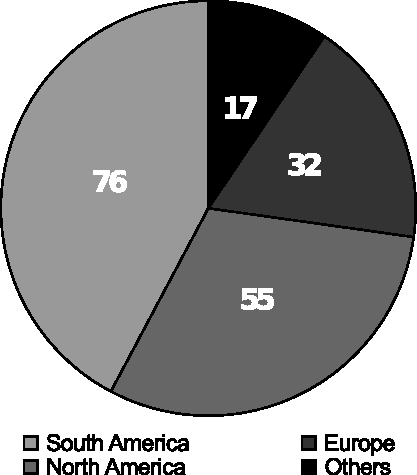
\includegraphics[scale=0.8]{floss-world.pdf}
    \caption{Answers by region of the world}
    \label{fig:floss-world}
  \end{minipage}
  \begin{minipage}[t]{0.5\linewidth}
    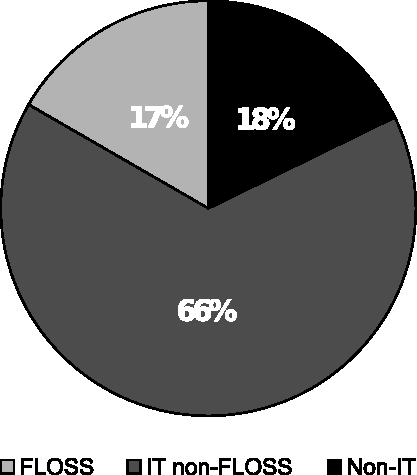
\includegraphics[scale=0.8]{floss-income.pdf}
    \caption{Main income origin}
    \label{fig:floss-income}
  \end{minipage}
\end{figure}

The analysis was performed over the 180 answers left since they
provided more interesting data. The figure \ref{fig:floss-world}
represents the distribution of the answers around the globe while the
figure \ref{fig:floss-income} shows the percentage main income origin
for the participants. The average age of the participants was 28 years
old and their first FLOSS contribution was around 22 years of age but
figure \ref{fig:floss-firstxp} shows that it the average first
contribution age for older people is higher than for younger ones.

\begin{figure}[htb]
  \centering
  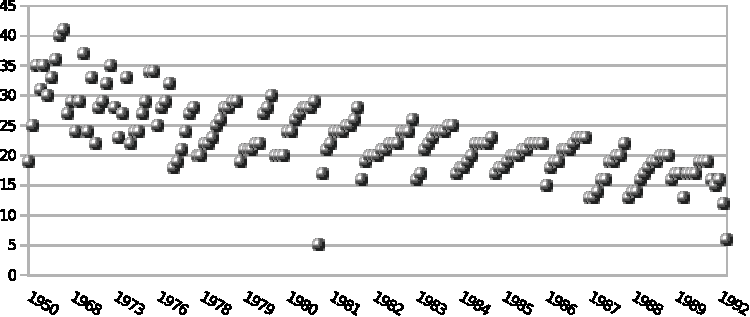
\includegraphics{floss-firstxp.pdf}
  \caption{Age of first contribution by year of birth}
  \label{fig:floss-firstxp}
\end{figure}

About two thirds of the participants were project maintainers,
commiters or programmers. The last third was partitioned between other
roles. So it looks like the sample is fairly good.

Regarding team sizes, only 6\% of the project were single person team
while 48\% were up to 5 team members. The rest of the projects were
evenly distributed between teams up to 10 members, from 11 to 50 and
more than 50.

\subsection{Individual results from the Agile community}
\label{subsec:agile-results}

Results were collected between 2009/10/01 and 2009/12/01.

\subsection{Crossed results}
\label{subsec:crossed-results}

\section{Conclusion}
\label{sec:conclusion}


\subsubsection*{Acknowledgments.}

This work was supported by the QualiPSo project \cite{url:qualipso}.

\begin{thebibliography}{5}

\bibitem{report:dempsey1999} Bert J Dempsey and Debra Weiss and Paul
  Jones and Jane Greenberg: A quantitative profile of a community of
  open source Linux developers (1999)

\bibitem{url:agilemanifesto} Kent Beck and Alistair Cockburn and Ward
  Cunningham and Martin Fowler and Ken Schwaber and al.: Manifesto for
  Agile Software Development, http://agilemanifesto.org (2001)

\bibitem{conference:oopsla2007} Dennis Mancl and Steven Fraser and
  William Opdyke: No silver bullet: a retrospective on the essence and
  accidents of software engineering (2007)

\bibitem{brooks1987} Frederick P. Brooks, Jr.: No Silver Bullet:
  Essence and Accidents of Software (1987)

\bibitem{gabriel2005} Ron Goldman and Richard P. Gabriel: Innovation
  Happens Elsewhere: Open Source as Business Strategy (2005)

\bibitem{XP2002} Kent Beck and Cynthia Andres: Extreme Programming
  Explained: Embrace Change, 2nd Edition (2004)

\bibitem{schwaber2004} Ken Schwaber: Agile Project Management with
  Scrum (2004)

\bibitem{cockburn2002} Alistair Cockburn: Agile Software Development
  (2002)

\bibitem{ohno1998} Taiichi Ohno: Toyota Production System: Beyond
  Large-Scale Production (1998)

\bibitem{poppendieck2005} Mary Poppendieck and Tom Poppendieck:
  Introduction to Lean Software Development (2005)

\bibitem{url:fowler2000orig} Martin Fowler: The New Methodology,
  http://martinfowler.com/articles/newMethodologyOriginal.html

\bibitem{fogel2005} Karl Fogel: Producing Open Source Software (2005)

\bibitem{url:flossproject} International Institute of Infonomics -
  University of Maastricht: Free/Libre/Open Source Software: Survey
  and Study - Report, http://www.flossproject.org/report/

\bibitem{url:flossdata} International Institute of Infonomics -
  University of Maastricht: Free/Libre/Open Source Software: Survey
  and Study - Report, http://www.flossproject.org/floss1/stats.html

\bibitem{reis2003} Christian Robottom Reis: Caracteriza\c{c}\~{a}o de
  um Processo de Software para Projetos de Software Livre (2003)

\bibitem{raymond1999} Eric S. Raymond: The Cathedral \& the Bazaar:
  Musings on {Linux} and Open Source by an Accidental Revolutionary
  (1999)

\bibitem{crowston2002} Kevin Crowston and Barbara Scozzi: Open source
  software projects as virtual organisations: competency rallying for
  software developement (2002)

\bibitem{fitzgerald2000} Joseph Feller and Brian Fitzgerald: A
  framework analysis of the open source software development paradigm
  (2000)

\bibitem{cockburn2004} Alistair Cockburn: Crystal Clear: A
  Human-Powered Methodology for Small Teams (2004)

\bibitem{oram2007} Andy Oram: Why Do People Write Free Documentation?
  Results of a Survey (2007)

\bibitem{riehle2007} Dirk Riehle: The Economic Motivation of Open
  Source Software: Stakeholder Perspectives (2007)

\bibitem{sutherland2007} Jeff Sutherland and Anton Viktorov and Jack
  Blount and Nikolai Puntikov: Distributed Scrum: Agile Project
  Management with Outsourced Development Teams (2007)

\bibitem{maurer2002} Frank Maurer: Supporting Distributed Extreme
  Programming (2002)

\bibitem{url:beck2008} Kent Beck: Tools for Agility,
  http://www.microsoft.com/downloads/details.aspx?FamilyID=ae7e07e8-0872-47c4-b1e7-2c1de7facf96
  (2008)

\bibitem{nagappan2003} Nachiappan Nagappan and Prashant Baheti and
  Laurie Williams and Edward Gehringer and David Stotts: Virtual
  Collaboration through Distributed Pair Programming (2003)

\bibitem{url:north2006} Dan North: Behaviour Driven Development,
  http://dannorth.net/introducing-bdd

\bibitem{sato2007} Danilo Sato and Alfredo Goldman and Fabio Kon:
  Tracking the Evolution of Object-Oriented Quality Metrics on Agile
  Projects (2007)

\bibitem{surowiecki2004} J. Surowiecki: The Wisdom of Crowds: Why the
  many are smarter than the few and how collective wisdom shapes
  business, economies, societies, and nations (2004)

\bibitem{tapscott2006} Don Tapscott and Anthony D. Williams:
  Wikinomics: How Mass Collaboration Changes Everything (2006)

\bibitem{benkler2006} Yochai Benkler: The Wealth of Networks: How
  Social Production Transforms Markets and Freedom (2006)

\bibitem{url:qualipso} Qualipso | Trust and Quality in Open Source
  systems, http://www.qualipso.org/

\end{thebibliography}

\end{document}
